% include the figures path relative to the master file
\graphicspath{ {./content/method/figures/visual_cues/}{./content/method/figures/}}

\section{Description of the segmentation methodology}\label{sec:method}

Optimization methodologies offer a standardized manner to approach segmentation by minimizing an application-driven cost function~\cite{cremers2007review}.
Figure~\ref{fig:method} illustrates a generic representation of the segmentation strategy, whereas concrete examples of its terms can be found in \cref{sec:methodApp} applied to \ac{bus}.
The overall segmentation can be seen as a three-steps strategy: 
(1) a mapping of the image into a discrete set of elements $\mathcal{S}$, 
(2) the optimization stage which is formulated as a \emph{metric labelling} problem, 
and (3) a re-mapping the labels obtained from the previous stage to produce the final delineation. 

\begin{figure}[htpb]
  \centering
  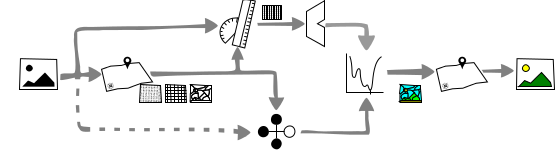
\includegraphics[width=0.9\linewidth]{method}
  \caption{Conceptual block representation of the segmentation methodology.}%\footnotemark}
    %\footnote{\cref{fig:methodTerms} illustrates the $\mathcal{S}$, $D(\cdot)$, and $V(\cdot)$ for the applied case of delineating breast structures in \ac{us} data.}
    %\footnote{(todo:add all the names of the elements in the figure)}
  \label{fig:method}
\end{figure}


In order to formulate the segmentation like a metric labelling problem, the image is conceived as a discrete set of elements $\mathcal{S}$ that need to be labelled using a label $l$ from the labelling set $\mathcal{L}$.
Let $\mathcal{W}$ be all the possible labelling configurations of the set $\mathcal{S}$, given $\mathcal{L}$.
Let $U(\cdot)$ be a cost function encoding the goodness of the labelling configuration $\omega \in \mathcal{W}$ based on the appearance of the elements in $\mathcal{S}$, their inner relation and some designing constraints.
Then, the desired segmentation $\hat{\omega}$ corresponds to the labelling configuration that minimizes this cost function, as described in Eq.\,\eqref{eq:costMin}.

\begin{equation}
\hat{\omega} = \arg \min_{\substack{\omega}} \,U(\omega)
\label{eq:costMin}
\end{equation}

\footnotetext{\Cref{fig:methodTerms} illustrates the $\mathcal{S}$, $D(\cdot)$, and $V(\cdot)$ for the applied case of delineating breast structures in \ac{us} data. {\color{red}(final version the figure elements should be labelled)}}

This goodness measure $U(\cdot)$ must be defined to take into account the appearance of the target region, its relation with other regions and other designing constraints.
Equation~\eqref{eq:labelingeq} describes this cost function as the combination of two independent costs that need to be simultaneously minimized as a whole.

\begin{equation}
  U(\omega) = \sum_{s\in \mathcal{S}} D_s(\omega_s) + \sum_{s \in \mathcal{S}}\sum_{r \in \mathcal{N}_{s}} V_{s,r}(\omega_s,\omega_r)
  \label{eq:labelingeq}
\end{equation}

Where, the left hand side of the expression integrates the so-called \emph{data} term, while the right hand side integrates the \emph{pairwise} term, which is also referred as the \emph{smoothing} term.
Both terms are shaped by $\mathcal{S}$ and evaluated in the labelling space $\mathcal{W}$.
%
In our quest to optimize the cost function $U(\cdot)$, it is required to define a representation for the set $\mathcal{S}$, a data term $D(\cdot)$, a pairwise term $V(\cdot)$, and a proper minimization methodology.

\paragraph{The set $\mathcal{S}$}
can be, in general, any discrete set representing the image (i.e.\, pixels, overlapping or non overlapping windows, super-pixels, etc.). 

\paragraph{The data term $D(\cdot)$,} \label{sec:method:dataTerm}
given a label configuration $\omega \in \mathcal{W}$, penalizes the labelling of a particular image element or site ($\omega_s = l$) based on the data associated to $s$.
In this manner, $D_s(\omega_s=l_\cmark) << D_s(\omega_s=l_\xmark)$.
Figure~\ref{fig:methodTerms}b illustrates the data cost associated to some arbitrary labelling configurations to clarify the desired effect (or behaviour) of this data term.
Designing an obscure heuristic to comply with the desired behaviour of $D(\cdot)$ out of the box, is rather a complicated task.
Therefore, an easier and cleaner approach is to design this data term $D(\cdot)$ with the help of \ac{ml} because it provides a systematic process that is flexible enough to encode any desired behaviour based on a training stage.
This concept is in fact depicted in the upper row in Fig.\,\ref{fig:method}.
For each site $s \in \mathcal{S}$, features describing $s$ are designed. Then, different optional steps can be applied to this set of feature: (i) features normalization, (ii) features selection or (iii) features extraction. Finally, the data term $D(\cdot)$ is encoded based on \ac{ml} classifiers, the features and a training step.
Thus, the data term $D(\cdot)$ can be seen as a distance or goodness measure reflecting the likelihood for $s$ to belong to class $l$.

\paragraph{The pairwise term $V(\cdot,\cdot)$} \label{sec:method:mrfTerm}
%The pairwise term 
represents the cost associated to $\omega_s$ taking into account the labels of its neighbour sites, $\omega_r$, $r \in \mathcal{N}_{s}$. 
This term models a \ac{mrf} or a \ac{crf}.
The typical form of this term, given in Eq.\,\eqref{eq:smoothing}, is called homogenization which acts as a regularization factor favouring configurations that have a coherent labelling.

\begin{equation}
V_{s,r}(\omega_s,\omega_r) = 
\begin{cases}
    \beta, & \text{if } \omega_s \ne \omega_r\\
    0,              & \text{otherwise}
\end{cases}
\label{eq:smoothing}
\end{equation}

Figure~\ref{fig:methodTerms}c shows a visual interpretation of this cost.
The more fragmented is the segmentation $\omega$, the higher the overall pairwise term; since every boundary brings a penalization $\beta$ to the total cost $U(\omega)$.
In this manner the regularization term can be seen as a post-processing or denoising stage since that some sites will flip their labelling if the cost of fragmenting the regions is larger than the cost of adopting their neighbour's label. 

% Review %contribute have different or variable costs (see \cref{fig:methodTerms:boundary}) are also possible by taking into account not only relations in $\mathcal{S}$ of but also image information (see \cref{fig:method}). 
%Further details can be found in \cref{sec:smoothing}.

\paragraph{The minimization strategy} \label{sec:method:min}
is determined by the nature of $U(\cdot)$ and $\mathcal{W}$, since not all the minimization strategies are applicable or adequate to find $\hat{\omega}$.
The size of the labelling space $|\mathcal{W}|=|\mathcal{L}|^{|\mathcal{S}|}$, discontinuities in $U(\omega)$ due to $\mathcal{W}$ or the problem of local minima, 
along with all the particular constrains of all the different minimization methodology.
Need to be taken into account while choosing the most desirable minimization strategy.

\begin{figure}[t]
    \centering
    \begin{subfigure}[b]{0.19\textwidth}
        \centering
        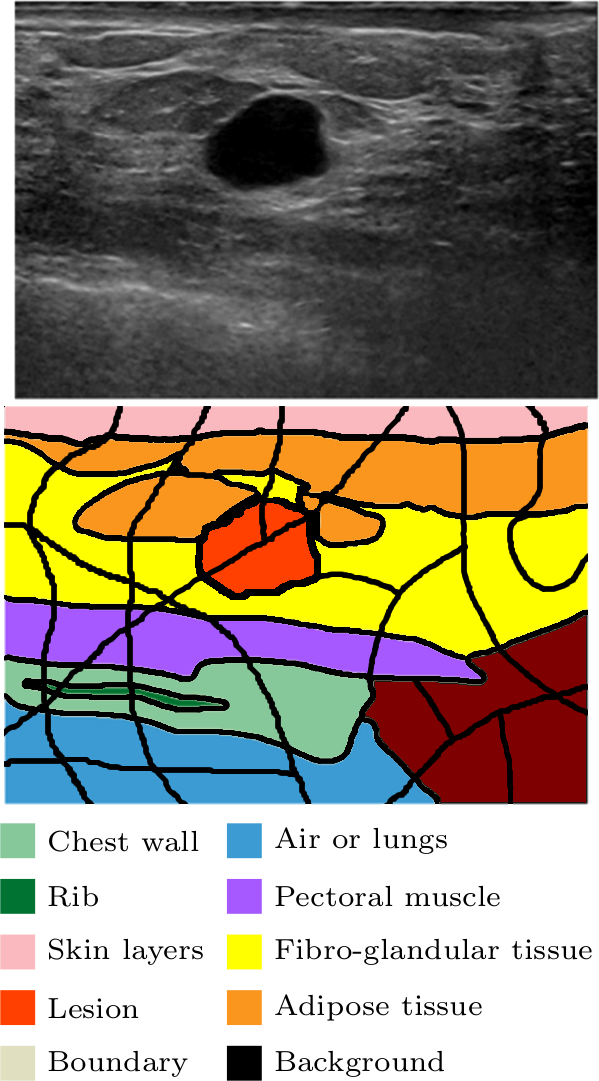
\includegraphics[width=\textwidth]{problem}
        %\caption{{\small Problem definition}}    
        \label{fig:methodTerms:problem}
    \end{subfigure}
    \hfill
    \begin{subfigure}[b]{0.39\textwidth}  
        \centering 
        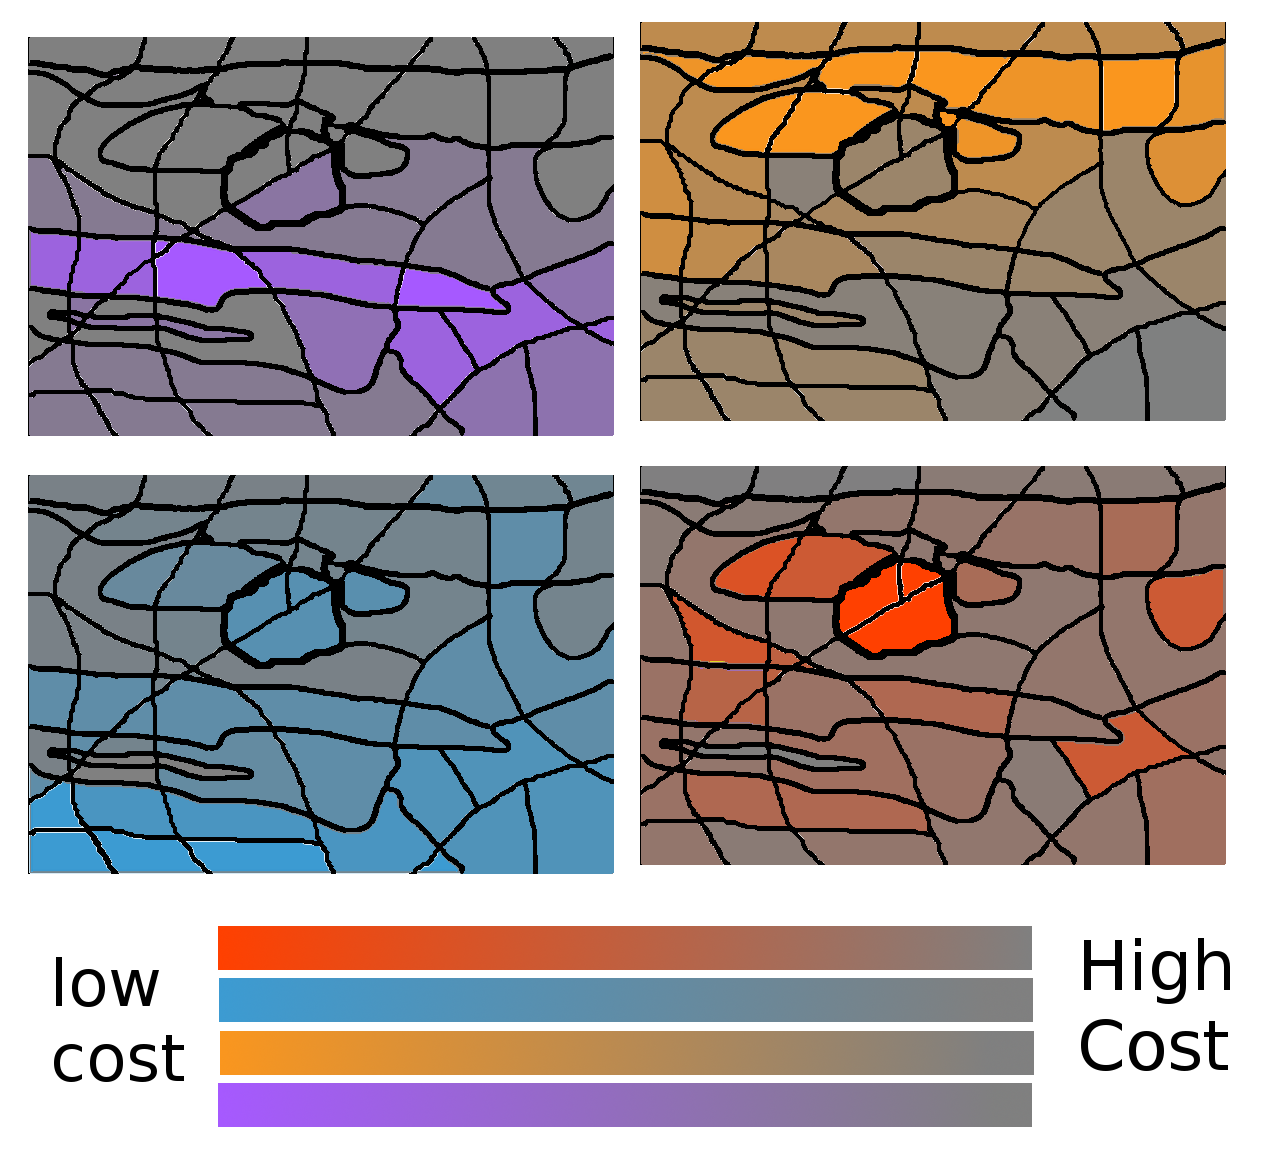
\includegraphics[width=\textwidth]{data}
        %\caption[]% {{\small Data term}}    
        \label{fig:methodTerms:data}
    \end{subfigure}
    \hfill
    \begin{subfigure}[b]{0.39\textwidth}   
        \centering 
        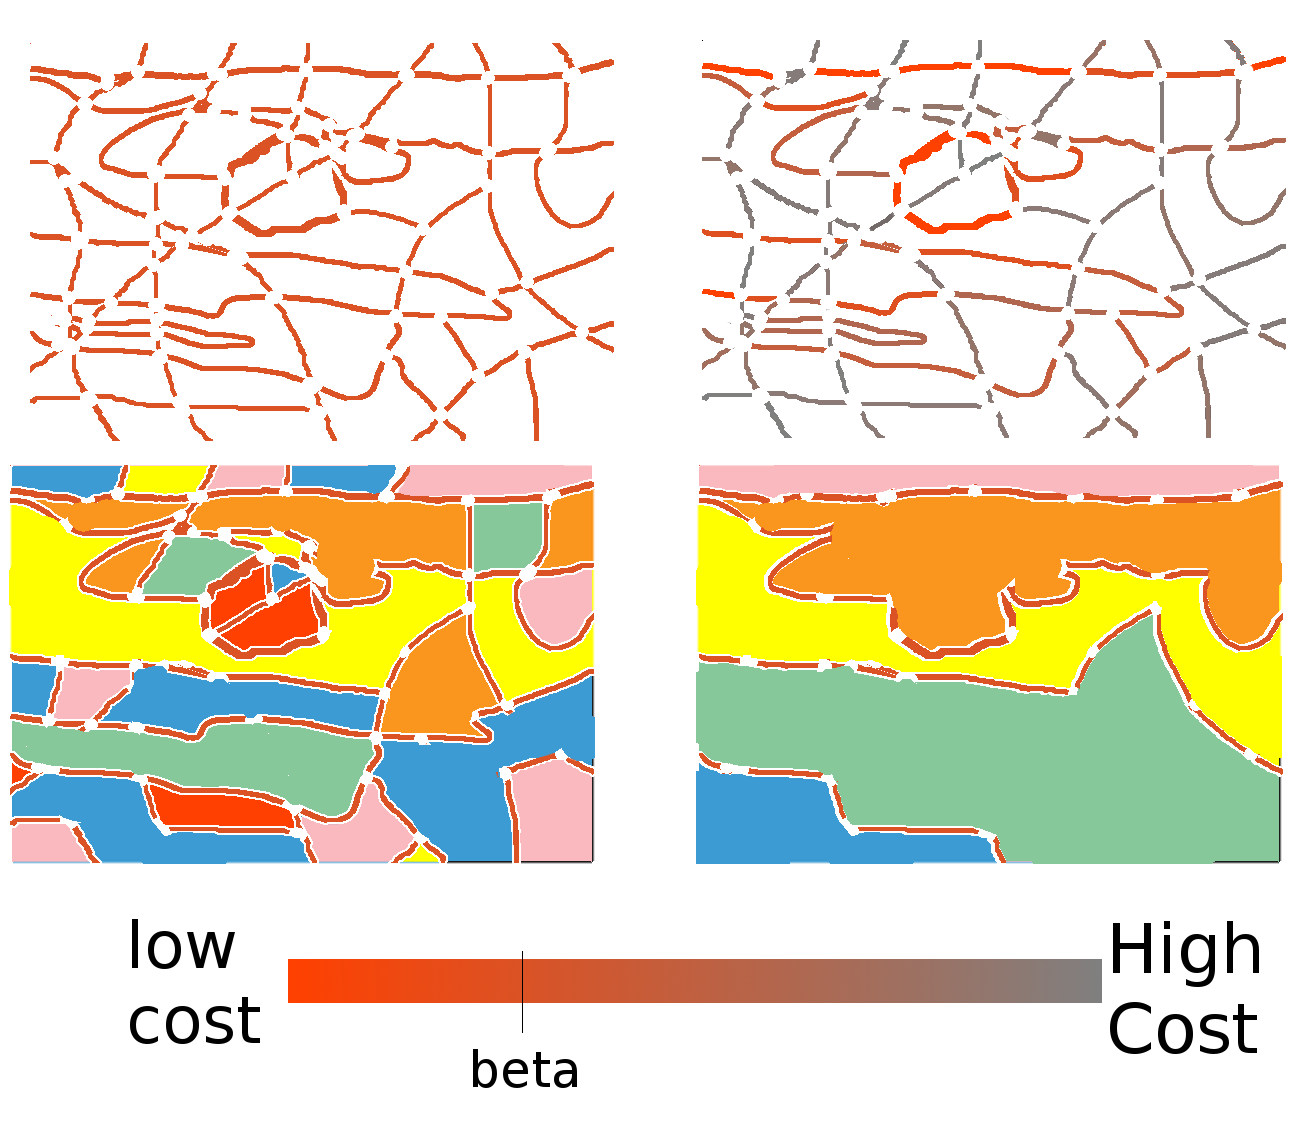
\includegraphics[width=\textwidth]{smooth} 
        %\caption[]% {{\small Pairwise term }}
        \label{fig:methodTerms:boundary}
    \end{subfigure}
    \caption {\small Methodology: (a) Problem definition, (b) Data term, (c) Pairwise term.} 
    \label{fig:methodTerms}
\end{figure}

%%% Local Variables: 
%%% mode: latex
%%% TeX-master: "../../master.tex"
